
% Based on the JuliaCon proceedings template
% Layout inspired by the International Journal of Computer Applications template
\documentclass{juliacon}
\usepackage{hgblistings}
\usepackage[many]{tcolorbox}
\usepackage[framemethod=tikz]{mdframed}
\lstMakeShortInline[language=Julia,columns=fixed]|
\setcounter{page}{1}

\newtcolorbox{calloutbox}[1][]{
  breakable,
  freelance,
  title=#1,
  colback=lightgray,
  colbacktitle=lightgray,
  coltitle=black,
  fonttitle=\bfseries,
  bottomrule=0pt,
  boxrule=0pt,
  colframe=lightgray,
  overlay unbroken and first={
  \draw[gray!75!black,line width=3pt]
    ([xshift=5pt]frame.north west) --
    (frame.north west) --
    (frame.south west);
  \draw[gray!75!black,line width=3pt]
    ([xshift=-5pt]frame.north east) --
    (frame.north east) --
    (frame.south east);
  },
  overlay unbroken app={
  \draw[gray!75!black,line width=3pt,line cap=rect]
    (frame.south west) --
    ([xshift=5pt]frame.south west);
  \draw[gray!75!black,line width=3pt,line cap=rect]
    (frame.south east) --
    ([xshift=-5pt]frame.south east);
  },
  overlay middle and last={
  \draw[gray!75!black,line width=3pt]
    (frame.north west) --
    (frame.south west);
  \draw[gray!75!black,line width=3pt]
    (frame.north east) --
    (frame.south east);
  },
  overlay last app={
  \draw[gray!75!black,line width=3pt,line cap=rect]
    (frame.south west) --
    ([xshift=5pt]frame.south west);
  \draw[gray!75!black,line width=3pt,line cap=rect]
    (frame.south east) --
    ([xshift=-5pt]frame.south east);
  },
}


\begin{document}

\title{Basic Threading Examples in JuliaLang v1.3}

\author[1]{Jameson Nash}
\author[1]{Jeff Bezanson}
\author[2]{Kiran Pamnany}
\affil[1]{Julia Computing, Inc.}
\affil[2]{Intel Corporation}

\keywords{Julia, JuliaLang, Multithreading, Parallelism, Concurrency, Optimization, Compiler, Runtime VM}


\maketitle

\begin{abstract}

A major distinguishing point of any programming language is how it deals with concurrency. Of course, I'm really interested here in parallelism, and specifically how to get the best throughput out of my application. But we know that actually taking advantage of all cores correctly and efficiently is really hard as a programmer. Here we take a look at how JuliaLang prepares to unleash the full power of your modern CPU's many cores.

Hopefully we won't drive any users mad with frustration as they try to write code to utilize threads. Towards that end, we'll look at how JuliaLang looks to provide a range of modern primitives that are designed to automatically compose effectively, and some of the trade-offs we make to try to simplify the mental model for the user. We'll also take a look at where we think that this development should go towards next.


\end{abstract}

\section{Introduction}
\label{subsub:intro}

A design principle for JuliaLang is to make common tasks easy and difficult tasks possible. This has extended from automatic memory management vs manual memory reuse, to having one type of method with dispatch, to optional type-inference for performance. And now, this includes concurrency. By extending design work that has been present in the language for many years to provide parallelism, we developed a means to add parallelism that preserved the (relative) simplicity of single-threaded for existing code, while allowing new code to benefit from the possibility of threading. This work has been inspired by parallel programming systems like Cilk, Intel Threading Building Blocks (TBB) and Go.

In this paradigm, any piece of a program can be marked for execution in parallel, and a “task” will be started to run that code automatically on an available thread. A dynamic scheduler handles making cache-aware decisions for when to launch the work items. This model of parallelism has many wonderful properties. We see it as somewhat analogous to garbage collection: with GC, you freely allocate objects without worrying about when and how they are freed. With task parallelism, you freely spawn tasks—potentially millions of them—without worrying about where they may eventually run.

The model is portable and free from low-level details. You don’t need to explicitly start and stop threads, and you don’t even need to know how many processors or threads there are (though you can find out if you want).

The model is nestable and compose-able: you can start parallel tasks that call library functions that themselves start parallel tasks, and everything works. This property is crucial for a high-level language where a lot of work is done by library functions. You need to be free to write whatever code you need—including parallel code—without worrying about how the libraries it calls are implemented. This model isn't limited just to JuliaLang code either: we've shown it can be extended to native libraries such as FFTW and are working on extending it to OpenBLAS.


\subsection{Background History}
\label{subsub:background}

Initially, JuliaLang exclusively provided users the ability to use cooperatively scheduled workers. In other contexts, these may be known as ``green threads'', ``threadlets'', or ``coroutines''. In Julia, we've called these tasks. A task is a unit of work with it's own context (stack) whose execution can be interleaved with that of any other task. Additionally, these have the ability to produce a value or an exception, making them useful for structured concurrency, without requiring an extra channel to manage. But they haven't had the ability to work in parallel (simultaneously).

These have been good for writing generators and outstanding for dealing with I/O workloads. In these cases, we know we might have a lot of unpredictable latency, so we need to be able to quickly jump between various threads of operation. When an event comes in, we need to resume our context quickly to react to the event before going off to handle something else. For example, a common pattern for a server is to provide a separate context for each child. Let's look at some code snippets for a toy socket echo server in a few other languages. With JavaScript promises, we could make something like the following work:

\begin{lstlisting}[language = JavaScript]
while (true) {
    listen(port)
        .then(client => {
            return client.read()
                .then(data => {
                    return client.write(data);
                })
                .then(() => {
                    return client.close();
                })
                .done();
        })
        .done();
};
\end{lstlisting}

With async/await we can make that a bit clearer with better structure and cut that down:
\begin{lstlisting}[language = JavaScript]
(async () => {
    while (true) {
        let client = await listen(port);
        (async () => {
            let data = await client.read();
            await client.write(data);
            await client.close();
        })();
    }
})();
\end{lstlisting}

But we still have some slightly obnoxious syntax there creating some distracting line noise. While most parts of the language are loosely typed and inferred by the runtime, this distinction is forced upon the user. So then, let's see how we would write that in Julia:

\begin{lstlisting}[language = Julia]
# function accept(cb, server)
#    while true
#        let client = accept(server)
#            @async cb(client)
#        end
#    end
# end
accept(listen(port)) do client
    data = read(client)
    write(client, data)
    close(client)
end
\end{lstlisting}

Notice here how we would typically leverage the do-block syntax to additionally re-use the loop logic, Task allocation, and error handling from a central place.

This works well for latency-bound activities, such as a web-server. But these codes only used one core, even though they only need to do thread-local actions, and so running these simultaneously on multiple threads should not require major changes. But also a lot of code is not written with the expectation of concurrent access, so we wanted to continue providing both kinds of concurrency. If we define a thread as a unit of work managed by the runtime system, we can call this $N:1$ threading, where the runtime library lets you manage N independent operations and maps them onto one system thread (approximately representing a CPU core). In the new system, we'll let the user now additionally have M CPU cores. This goes beyond the classic $N:M$ threading model however, as you have cooperative affinities where certain tasks won't interrupt each other. I propose calling this $N(k:1):M$ scheduling since we're combining the advantages of single-threaded work queues with multiple cores.

In $N(k:1):M$ scheduling, we have N units of work mapped onto M cpu threads. Additionally, each of those units of work may be composed of k cooperatively scheduled Tasks. This is achieved by pinning the tasks in the group to one CPU-thread, while load balancing those across the available cores using the novel partr scheduler algorithm. Finally, we can extend this model once more by factoring out a common factor of $P:P$ to write this as $N(k:1):M+P(k:1):P$ and derive one further useful use case: the ability to pin one thread to running one task (or task-group). These P tasks could be an over-subscription of the CPU cores, or take away from M, or both. Typical uses for this mode of operation would be high-availability tasks (with low latency requirements, but also minimal computation), such as background I/O processing, blocking work pools (foreign library integration), finalizers, or message server queues.

The newest work here is to implement a thread-aware scheduler. For a couple years, JuliaLang has been able to perform simple tasks with some caveats with a static work schedule and minimal-to-none inter-thread communication. This had been given the status of ``experimental,'' while we worked out the details and shook out the bugs. The recent work to generalize that functionality has allowed us to rewrite that older static capability on top of our new runtime, demonstrating the power and flexibility of the new system. While the old system let us test out the thread-related bugs in the runtime, it had some significant shortcomings. We knew those would need to be addressed before we could move beyond the ``experimental'' label.

Those limitations included:
\begin{itemize}
\item it had no scheduler, and so couldn't interact with regular tasks or do I/O
\item the runtime was full of race conditions
\item the `\verb|@threads|' loops could not be nested
\item parallel code couldn't run outside the `\verb|@threads|' loop
\end{itemize}

\begin{calloutbox}[Running Julia with Threads]
In the examples below, we will be using JuliaLang v1.3 launched with multiple threads.
To get follow along on your own machine, you will want to download the upcoming JuliaLang release (currently v1.3.0-rc1) from \url{https://julialang.org/downloads}.
Run \verb|./julia| with the environment variable \verb|JULIA_NUM_THREADS=| set to the number of threads to use.

Alternatively, after installing JuliaLang, follow the steps at \url{http://docs.junolab.org/latest/man/installation/} to install the \href{https://junolab.org}{Juno IDE}. It will automatically set the number of threads based on the number of available processor cores, and also provides a graphical interface for changing the number of threads.
\end{calloutbox}

\section{Motivating Examples}
\label{subsub:motivation}

The presence and usability aspects of threading, as exemplified here, reflect JuliaLang's general policy of giving users control. One driving philosophy is that users should have the \textit{ability} to access the full power of their machine. And it should be easy when needed but ignorable when not required.

While many, or even most, programs can be written without needing to touch multithreading, some require them, while some benefit from them. In this paper, we'll primarily examine some cases where threads aren't required, but are improved by their presence. Additionally we'll look at a case where the work can be run sequentially with cooperative scheduling, but at greatly reduced performance.

Most thread-specific functionality is exported from the \verb|Threads| submodule of the \verb|Base| module. For example, we can querying it for the runtime number of threads and the id of the current thread:

\begin{lstlisting}[language = Julia]
julia> Threads.nthreads()
4

julia> Threads.threadid()
1
\end{lstlisting}

\subsection{Stochastic Ordering}
\label{subsub:pprint}

One of the more visual ways to show we have threads working is to show the scheduler picking up work in semi-random, interleaving, orders. Previous versions of Julia already had an `\verb|@threads for|' macro which would split a range and run a portion on each thread with a static schedule. So in the range below, thread 1 would run items 1 and 2, thread 2 would run items 3 and 4, and so on. Now these threads supports doing I/O too with that same schedule.

\begin{lstlisting}[language = Julia]
bash$> JULIA_NUM_THREADS=8 julia <<EOF
Threads.@threads for i = 1:12
    println(i, " on thread ", Threads.threadid())
end
EOF
1 on thread 1
3 on thread 2
12 on thread 8
9 on thread 5
7 on thread 4
2 on thread 1
4 on thread 2
5 on thread 3
8 on thread 4
11 on thread 7
10 on thread 6
6 on thread 3
\end{lstlisting}

But now, it's also now possible to do the same example but with a completely dynamic schedule. With the improved language runtime, this takes a few small tweaks now. We use the new `\verb|@spawn|' macro with the existing `\verb|@sync|' macro to delineate the work items.

\begin{lstlisting}[language = Julia]
bash$> JULIA_NUM_THREADS=8 julia <<EOF
@sync for i = 1:12
    Threads.@spawn println(i, " on thread ", Threads.threadid())
end
EOF
2 on thread 5
3 on thread 4
8 on thread 7
6 on thread 5
12 on thread 7
7 on thread 6
9 on thread 8
10 on thread 5
4 on thread 3
1 on thread 2
5 on thread 1
11 on thread 1
\end{lstlisting}

But on to even more fun stuff...

\subsection{Parallel Merge Sort}
\label{subsub:psort}

A classic algorithm, parallel merge sort shows nice performance benefit and scaling from using multiple threads. This function will create $O(log(n))$ subtasks which will sort independent portions of the array before merging them into a final sorted copy of the input. We use here the ability of each task to return a value to directly \verb|fetch| the result without requiring an additional channel for data!

\begin{lstlisting}[language = Julia]
# perform a merge sort on `v` using parallel threads
function psort(v::AbstractVector)
    hi = length(v)
    if hi < 100_000 # below some cutoff, run in serial
        return sort(view(v, 1:hi), alg = MergeSort)
    end
# split the range and sort the halves in parallel recursively
    mid = (1 + hi) >>> 1
    half = Threads.@spawn psort(view(v, 1:mid))
    right = psort(view(v, (mid + 1):hi))
    left = fetch(half)::typeof(right)
# perform the merge on the result
    out = similar(v)
    i, il, ir = 1, 1, 1
    @inbounds while il <= mid && ir <= (hi - mid)
        l, r = left[il], right[ir]
        if l < r
            out[i] = l
            il += 1
        else
            out[i] = r
            ir += 1
        end
        i += 1
    end
    @inbounds while il <= length(left)
        out[i] = left[il]
        il += 1
        i += 1
    end
    @inbounds while ir <= length(right)
        out[i] = right[ir]
        ir += 1
        i += 1
    end
    return out
end
\end{lstlisting}

To see the timing results as we add threads, refer to figure \ref{fig:scalings} at the end.

While not demonstrated here, \verb|fetch| would also automatically propagate errors, with the result of it being an error thrown if the child task ended by throwing an exception.

Since we are using in-process threads, we could further optimize this to instead mutate the input in-place and to reuse work buffers for additional performance. We have elsewhere tested that and shown the performance improvement is as expected. However, since the scaling improvement was similar between them, we've opted not to include it here.

\subsection{Parallel Primes Sieve}
\label{subsub:pprimes}

An unusual use of high-level threading operations can be used to (inefficiently) compute prime numbers using the sieve of Eratosthenes.
This use of threaded channels is translated from Thomas Hoare's seminal 1978 paper ``Communicating Sequential Processes''\cite{Hoare:1978:CSP:359576.359585} example 6.1. It works by creating a task for each prime number being generated. Upon receiving (and outputing) a prime, each task will then take responsibility for filtering out multiples of that prime from the input list, as represented in figure \ref{fig:sieve}.

\begin{figure}[ht]
\centerline{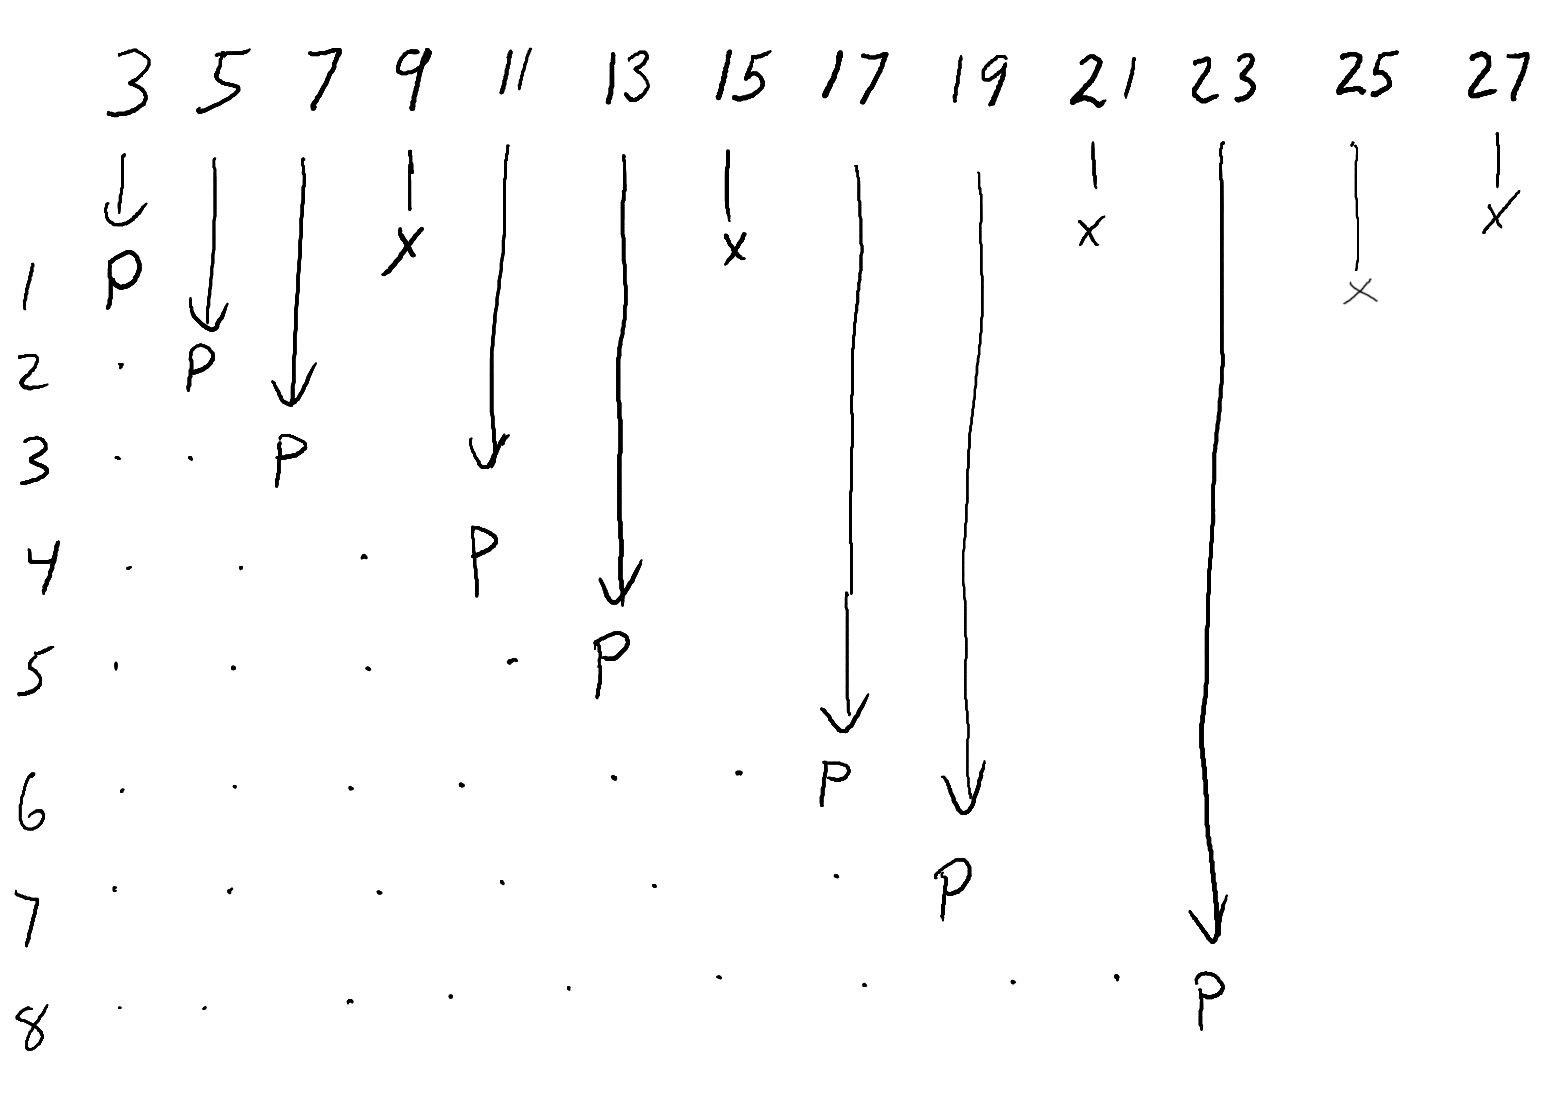
\includegraphics[width=6cm]{images/threads_sieve.png}}
\caption{Primes sieve in operation. Inputs `$n$' across the top. Task numbers `$i$' down the side. Outputs `$P$' marked in the center.}
\label{fig:sieve}
\end{figure}

\begin{lstlisting}[language = Julia]
function S61_SIEVE(n::Integer)
    buffer = 5 # buffer capacity (configurable)
    primes = Int[] # result
    done = Threads.Atomic{Bool}(false) # completion signal
    sieves = [Channel{Int}(buffer) for i = 1:n]
    for i in 1:n
        Threads.@spawn begin
            p = take!(sieves[i])
            push!(primes, p)
            if length(primes) == numPrimes
                done[] = true
                return
            end
            mp = p # non-prime multiples of p
            for m in sieves[i]
                while m > mp
                    mp += p
                end
                if m < mp # rem(m, p) > 0
                    put!(sieves[i + 1], m)
                end
            end
        end
    end

    put!(sieves[1], 2)
    n = 3
    while !done[]
        put!(sieves[1], n)
        n += 2
    end
    return primes
end
\end{lstlisting}

To see the timing results as we add threads, refer to figure \ref{fig:scalings} at the end.

Since we're creating one thread for each number, the overhead here overwhelms the computational cost of the additions. That makes this implementation \textit{much} slower than the optimized routines typically used now, such as those provided in \verb|Primes.jl| to compute \verb|primes|. But is also means we show exceptional (super-linear) scaling. This is because we end up being able to run a better schedule when we can fill and empty the channels in parallel. That is also why the presence of at least a small buffer on the channel can be a significant advantage for the implementation.

\subsection{Parallel Prefix Scan}
\label{subsub:ppscan}

Prefix-scan-sum is another classic algorithm that is able to benefit nicely from having multiple threads. Without going into any details about how this operation works or what it does, the short code below can take advantage of all cores and SIMD units available on the native machine—even with a generic ahead-of-time-compiled system image:

\begin{lstlisting}[language = Julia, inputencoding=utf8, literate = {⊕}{{$\oplus$}}1]
using .Threads: @threads
function prefix_threads!(⊕, y::AbstractVector)
    l = length(y)
    k = ceil(Int, log2(l))
    # do reduce phase
    for j = 1:k
        @threads for i = 2^j:2^j:min(l, 2^k)
            @inbounds y[i] = y[i - 2^(j - 1)] ⊕ y[i]
        end
    end
    # do expand phase
    for j = (k - 1):-1:1
        @threads for i = 3*2^(j - 1):2^j:min(l, 2^k)
            @inbounds y[i] = y[i - 2^(j - 1)] ⊕ y[i]
        end
    end
    return y
end

A = fill(1, 500_000)
prefix_threads!(+, A)
\end{lstlisting}

JuliaLang can express this operation so well because it defines an expressive front-end to describe optimizations to the compiler. Under the hood, it puts together a comprehensive set of features that free the user from dealing with memory management, thread management, nor compile/runtime distinction. The runtime is able to prepare a version of this function specifically optimized for the arguments types. And it spawns closures to be run on all available CPUs. The compiler can also automatically specialize the function for the current processor (both ahead-of-time and just-in-time), adjusting the ABI on-the-fly (with trampolines as needed). And our lightweight threading system will dynamically schedule the work chunks.

\section{Performance}
\label{subsub:performance}

Each of the examples above shows a performance benefit attained from adding threads!

On my quad-core laptop (Intel(R) Core(TM) i7-8559U CPU @ 2.70GHz), I obtained the following scaling and timing numbers shown in table \ref{table:timings} and \ref{table:scalings}.

\lstDeleteShortInline|
\begin{table}[ht]
\tbl{Measured timing of the examples given above.}{
\begin{tabular}{ |l l l l l| }
    \hline
    nthreads & 1 & 2 & 3 & 4 \\
    \hline
    S61\_SIEVE & .704s & .709s & .065s & .241s \\
    psort & .609s & .528s & .321s & .993s \\
    prefix\_threads! & .375s & .462s & .100s & .043s \\
    \hline
\end{tabular}}
\label{table:timings}
\end{table}

\begin{table}[ht]
\tbl{Timing figures from table \ref{table:timings} converted to scaling ratios relative to the first column.}{
\begin{tabular}{ |l l l l l| }
    \hline
    nthreads & 1 & 2 & 3 & 4 \\
    \hline
    S61\_SIEVE & 1x & 1.91x & 3.62x & 6.56x \\
    psort & 1x & 1.71x & 1.98x & 2.63x \\
    prefix\_threads! & 1x & 1.62x & 2.16x & 2.28x \\
    \hline
\end{tabular}}
\label{table:scalings}
\end{table}
\lstMakeShortInline[language=Julia,columns=fixed]|

These can be seen plotted graphically in figure \ref{fig:timings} and \ref{fig:scalings}.

\begin{figure}[ht]
\centerline{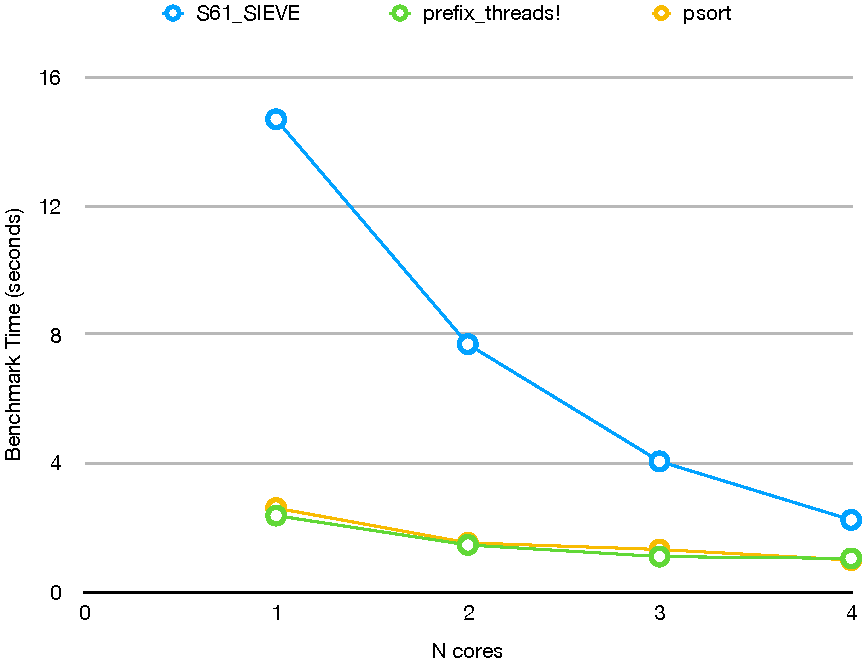
\includegraphics[width=6cm]{images/threads_timing.pdf}}
\caption{Timings from table \ref{table:timings} plotted graphically.}
\label{fig:timings}
\end{figure}

\begin{figure}[ht]
\centerline{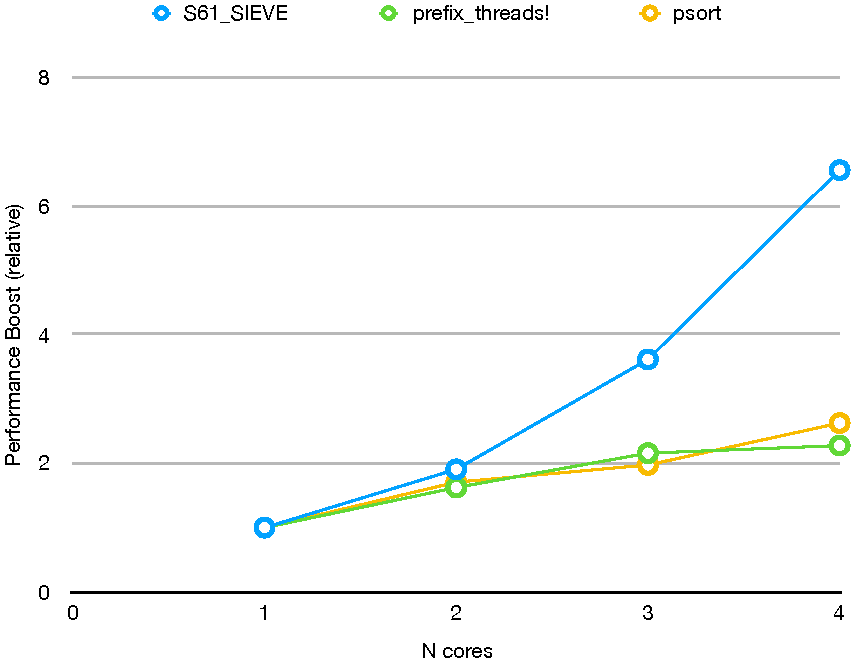
\includegraphics[width=6cm]{images/threads_scaling.pdf}}
\caption{Scaling ratios from table \ref{table:scalings} plotted graphically.}
\label{fig:scalings}
\end{figure}

\section{Integration into an existing language}
\label{subsub:integration}

Another challenge we faced was seeing what would be needed to integrate this work with pre-existing code. JuliaLang is an existing, post version 1.0 language with promises to maintain backwards compatibility and a large third-party code base that depends on it. Any changes needed to have an upgrade-path. Whenever there were existing code that might reasonably be expected to be safe to use from multiple threads, that code needed to be identified and fixed. Fortunately, many key aspects of the language had previously been designed in expectations of becoming threaded. In some other popular languages, we see they have not been able to add unrestricted threading. There were several areas that needed to be tackled to determine the appropriate upgrade path:

User-facing APIs:
\begin{itemize}
\item concurrency basics: \verb|Task|, and associated functions including \verb|schedule|, \verb|yield|, \verb|wait|
\item mutexes: \verb|ReentrantLock| and \verb|Condition| variables, including \verb|lock|, \verb|unlock|, \verb|wait|
\item synchronization primitives: \verb|Channel|, \verb|Event|, \verb|AsyncEvent|, \verb|Semaphore|
\item IO and other delays: including \verb|read|, \verb|write|, \verb|open|, \verb|close|, \verb|sleep|
\item experimental \verb|Threads| module: random assortment of building blocks and atomics
\item memoization-type caches (e.g. inside \verb|Regex.PCRE| and the \verb|Random.GLOBAL_RNG| object reference)
\end{itemize}

Once we determined we wanted to make concurrency and parallelism use the same concept (named a \verb|Task|), that set many priorities. Many of the APIs in our list of user-facing APIs were able to directly add thread-safety ``under-the-hood'', as they say. This meant that we found that typical user code that already interacted with IO, synchronization, locks, and tasks could continue to operate unchanged. In most cases, we achieved this by adding fine-grained locks on each critical resource. There were a few notable cases:

\subsection{Changes to Tasks}
\label{subsub:integration-tasks}

The existing concurrency primitive of \verb|Tasks| was enhanced by exposing a new, optional flag to enable thread-migration for it. We call this concept ``sticky'' tasks, as a default tasks is only cooperatively runnable on the thread that \verb|scheduled| them. When set to false, however, the task becomes eligible to be picked up by any other thread. Combined with the internal changes to make \verb|wait| on events and channels thread-safe, we believe this provides an easy-to-use mechanism for selecting between the simpler cooperatively concurrent usage (single-threaded) and the more general simultaneous parallelism (multi-threaded).

\begin{lstlisting}[language = Julia]
t = Task(() -> [closure code])
t.sticky = false # t may now get run on any thread
schedule(t)
...
wait(t)
\end{lstlisting}

However, while conceptually simple, the above felt slightly awkward compared to the fairly succinct \verb|@async| syntax used for creating a concurrent task. We wanted to make it similarly convenient, so we also created a new \verb|Threads.@spawn| macro and integrated it with the existing \verb|@sync| macro.

\begin{lstlisting}[language = Julia]
using Threads: @spawn
@sync begin
    @async concurrent_closure()
    @spawn parallel_closure()
end # wait for all
\end{lstlisting}

\subsection{Changes to Condition}
\label{subsub:integration-condition}

The existing \verb|Condition| object couldn't be made thread-safe. There were two replacements identified: one, replace it with an auto-resetting event with the same API; or two, replace it with a new mutex-based API. We decided to go with the latter option. This meant that existing usage of Condition was only correct if it remained on a single-thread. We decided to mechanically enforce this by asserting on usage that it was always used from the same thread it was created on. The new API requires writing the following more verbose code pattern:

\begin{lstlisting}[language = Julia]
c = Threads.Condition()
# or alternately
#   l = ReentrantLock()
#   ...
#   c1 = Threads.Condition(l)
#   c2 = Threads.Condition(l)
...
lock(c)
try
    while !is_condition_met()
        ...
        wait(c)
        ...
    end
finally
    unlock(c)
end
...
\end{lstlisting}

Previously, this would have been more simply |c = Condition(); is_condition_met() || wait(c)|.  While this change may seem more difficult at first glance, we observed that while the lock acquisition here could be hidden inside \verb|wait| in the first replacement, all of this structure will usually still be required by the |is_condition_met| function. And the code would get much further complicated by the need to release the lock before calling \verb|wait|. We concluded therefore that in most cases the code would be made simpler and faster by changing the API to the second option. This also meant that when code was being changed to be thread-safe, it would need to replace uses of \verb|Condition| with the new \verb|Threads.Condition|.

\subsection{Changes to IO}
\label{subsub:integration-io}

Changing the I/O code (files, streams, folders, and other platform code) to work on from any thread was another big project. The existing design requires an underlying asynchronous library, with a design similar to Windows IOCP, to efficiently manage large numbers of open event sources and provide the simplicity and concision of the logic shown in \ref{subsub:background} on all platforms. For this, we have been using the libuv library. This lets us have most platform-specific code isolated in a separately tested library and provide more commonality in our runtime library. As an initial implementation to make this library safe to use from threads, we've used one big IO lock around all calls to it. However, this library also has callbacks and will block to wait for external incoming events, so we also needed to integrate it fully with the task scheduler to get it to cooperatively release the lock on demand. We were able to do so by adding an asynchronous channel (\verb|uv_async_t|) to wake the one thread running the event loop while all other threads sleep on a system mutex (\verb|uv_cond_t|) when there is no work for them to perform. When try entering the event loop, we do so only if the count of currently waiting tasks is zero. In the future, this work may allow us to move the event loop entirely to a separate thread (and/or multiple threads). It seems that this design change may thus be making threading support a mandatory requirement for the underlying VM—with the advantage we that we can get more throughput on the large-core systems that are only becoming more common.

\subsection{Changes to Memoization Caches}
\label{subsub:integration-caches}

The usual strategy for dealing with these was to turn them from true globals into thread-local variables. To assist in that goal, we assign all threads a low numbered \verb|threadid|. This can then be used to index a global array to access the cache for that thread. For example, instead of one global \verb|Random.GLOBAL_RNG| object representing the global \verb|MersenneTwister| pseudo-random number generator (PRNG) state, we use a \verb|Random.default_rng()| function to retrieve the current PRNG for that thread (or to lazy-initialize one from system randomness on first use).

\begin{lstlisting}[language = Julia]
function default_rng()
    tid = Threads.threadid()
    @assert 0 < tid <= length(THREAD_RNGs)
    if @inbounds isassigned(THREAD_RNGs, tid)
        @inbounds MT = THREAD_RNGs[tid]
    else
        MT = MersenneTwister()
        @inbounds THREAD_RNGs[tid] = MT
    end
    return MT
end
function __init__()
    resize!(empty!(THREAD_RNGs), Threads.nthreads())
end
\end{lstlisting}


\subsection{Changes to the Julia Runtime Library}
\label{subsub:integration-runtime}

The functionality provided in libjulia also needed to be thread-safe. While some of it consists of stateless helper functions, much of it is where the shared global state for the language lives (by contrast, much of the system library is written in the JuliaLang language itself and as a general principle, the whole system has avoided using mutable global state unless essential).

Due to the design of the rest of the language avoiding access to mutable state inside the runtime library, we felt it would acceptable to use fine-grained locked for protecting most accesses. Many of these were added in an earlier version of JuliaLang, while threading was still under highly experimental development. These included such aspects as code-generation (JIT compilation) and GC (memory allocation and freeing).

Discussion of the GC design and subsequent updates to make it work well with threads could occupy an entire article of its own, so it will not be discussed here. Although in the future work section later in this paper, some improvements being investigated for the compiler will be discussed.

When using locks, there is a hierarchy of access that must be respected to avoid deadlocks. This is documented somewhat sparsely at \url{https://docs.julialang.org/en/v1/devdocs/locks/}. Over time, we'll extend this list as we discover problems or are able to simplify shared resources. There's some known issues already, such as the lack of a lock around certain ``toplevel-only'' operations and an invalid design for the ordering of the \verb|Module->lock|. These issues will be addressed in time—they are not known to be insurmountable issues.

The missing toplevel lock is interesting, since it is a lock against concurrent execution of \textit{any} other code. This will require halting all other threads in some way to inhibit accidental observation of the global state while it's in an intermediate inconsistent state. This should be possible in coordination with the GC-safepoint lock, which already has a very similar problem.

Some aspects were still too performance critical however to be able to use a lock there, so we also make careful use of atomic pointer-publishing updates in a few specific places. As special-cases of that, we use RCU-type (read-copy-update) updates in some places and write-once in other places). This is known to work on most computer architectures. Others, such as the notorious A, we are content to exclude. In a code-base that already supports garbage-collection, the RCU algorithm is greatly simplified (and writers pay no additional cost), so this is typically preferred, if mutation is absolutely required and reads must be fast. Otherwise, a simple lock is used.

\section{Implementation}
\label{subsub:implementation}

A prototype implementation of the \verb|partr| scheduler was first written for us in C by Kiran Pamnany of Intel back in late 2016, following research done on scheduling threads for beneficial cache sharing for best throughput\cite{Chen:2007:STC:1248377.1248396}. The goal of this work was effortless composition of threading-capable libraries with a globally depth-first work ordering (as opposed to $1:1$/preemptive scheduling, which would try to make progress on all work, or work-stealing scheduling, which is only depth-first local to a thread and is globally breadth-first).

The next stage of this work was then to integrate it with the existing JuliaLang runtime system and hoist as much of the implementation as possible into native Julian code. (Aside: one outcome of this work has been to allow us to delete much of the special support code from the C runtime for our prior experimental `\verb|@threads|' fork/join-style API!)

A big challenge of this work has been implementing a sound algorithm for determining when threads should ``park'' themselves in a sleep mutex or wait for IO. This requires careful coordination to ensure we don't create a single contention point when trying \verb|schedule| and run tasks, but also is responsive to resume when new work arrives (either internally, from another thread, or externally, from IO streams). This is done by setting a flag in the task to notify it after work is added to the queue. If the running task sees that the thread was previously sleeping, it then additionally notifies its condition variable to wake it up.

\section{Foreign Libraries}
\label{subsub:ffi}

An important motivation for this work was our desire to better support multi-threaded-capable libraries, without considerable CPU over-subscription killing performance due to cache-thrashing and frequent preemptive CPU context switches. Previously, the only options were often for the user to decide up-front to limit JuliaLang to N threads, and tell the threaded library (such as libfftw or libblas) use $\lfloor M \div N \rfloor$ (floordiv) cores. The most common choices probably being 1 and M, so only part of the application and running time is able to benefit from the presence of multiple cores in the system. However, given our ability to quickly create and run work items in our thread pool, we are looking at how to work with external libraries also and let them also integrate with our existing thread-pool.

This is an on-going area of exploration as we get feedback on the performance and API needs of various libraries.

We've successfully adapted FFTW to run on top of our threading runtime instead of its own (a pthreads-based workpool). This took us only a few hours! (We were fortunate to be able to enlist the assistance of that library's author). Without any performance tweaking (yet), it got competitive performance results! We learned important lessons in needing to tightly optimize our scheduler latency, which is now ongoing work to achieve exact performance parity. Even with some overhead imposed by generality, however, we expect that the ability to compose thread-aware users and enable the better resource sharing created by the partr scheduler will make this an overall improvement in program operation.

\section{Future work}
\label{subsub:future}

While this work has been ongoing for several years already, there's still much interesting or important improvements to consider. We'd like to investigate ways to further expand the thread-safe API surface and integrate powerful thread-sanitizer tooling to help users write better code. There's also substantial room for the standard library to start using this threading runtime whenever possible. But we need to yet experiment with ways to safely and conveniently expose this option to users (which often seem contradictory).

There also should be more performance testing to fine-tune the heuristic numbers. For example, when adding work items to the dynamic scheduler to run on $P$ cores, what is a good ratio factor $k$ to use when creating chunks of work? Should we make $1P$ items (assume a static schedule)? or $105P$ (assume a static schedule on either of $P$ or $P-1$ processors for $P=4,6,8,16$)? Or perhaps simply $3P$ is sufficient to balance out much variation? And yet other workloads, however, may want one work item for every input value (like \verb|Distributed.pmap| does)!

While I could mention many more items that remain to be explored, there's just one more I want to highlight: concurrent garbage collection. Currently, JuliaLang's runtime library needs to wait for all threads to arrive at a safe-point or be in a safe-region (such as foreign code) before GC can start. This can introduce long pauses if one or more threads are far away from hitting such a region. Presently, those only exist where manually inserted into the code, such as while waiting for a lock or doing allocation. In the future, it is proposed we investigate options for automatic placement of these by the system to minimize gc-start latency without unduly impacting allocation-free code. There are certainly more approaches to handle releasing memory then there are language implementations in existence, possibly multiple times over. So suffice to say this is an area with many possible trade-offs! For an example of where we might also go with this, please take a look at the \href{https://www.mono-project.com/docs/advanced/runtime/docs/coop-suspend/}{Mono project's documentation on cooperative thread suspension}\cite{mono-coop-suspend} for how a different language, which shares a common code-generation strategy, handles this.

\section{Conclusions and summary}
\label{subsub:conclusion}

JuliaLang's approach to multi-threading combines many previously known ideas in a novel framework. While we believe that each in isolation is useful, that—as is so often the case—the sum is more than the parts.

\section{Acknowledgements}
\label{subsub:acknowledgements}

The authors would like to gratefully acknowledge funding support from Intel and relationalAI that made it possible to develop these new capabilities.

We are also grateful to the several people who patiently tried this functionality while it was in development and filed bug reports or pull requests, and spurred us to keep going.


\section{Bad puns}
\label{subsub:puns}

We liken the addition of thread-safety as moving from the age of mechanization...

\begin{figure}[h]
\centerline{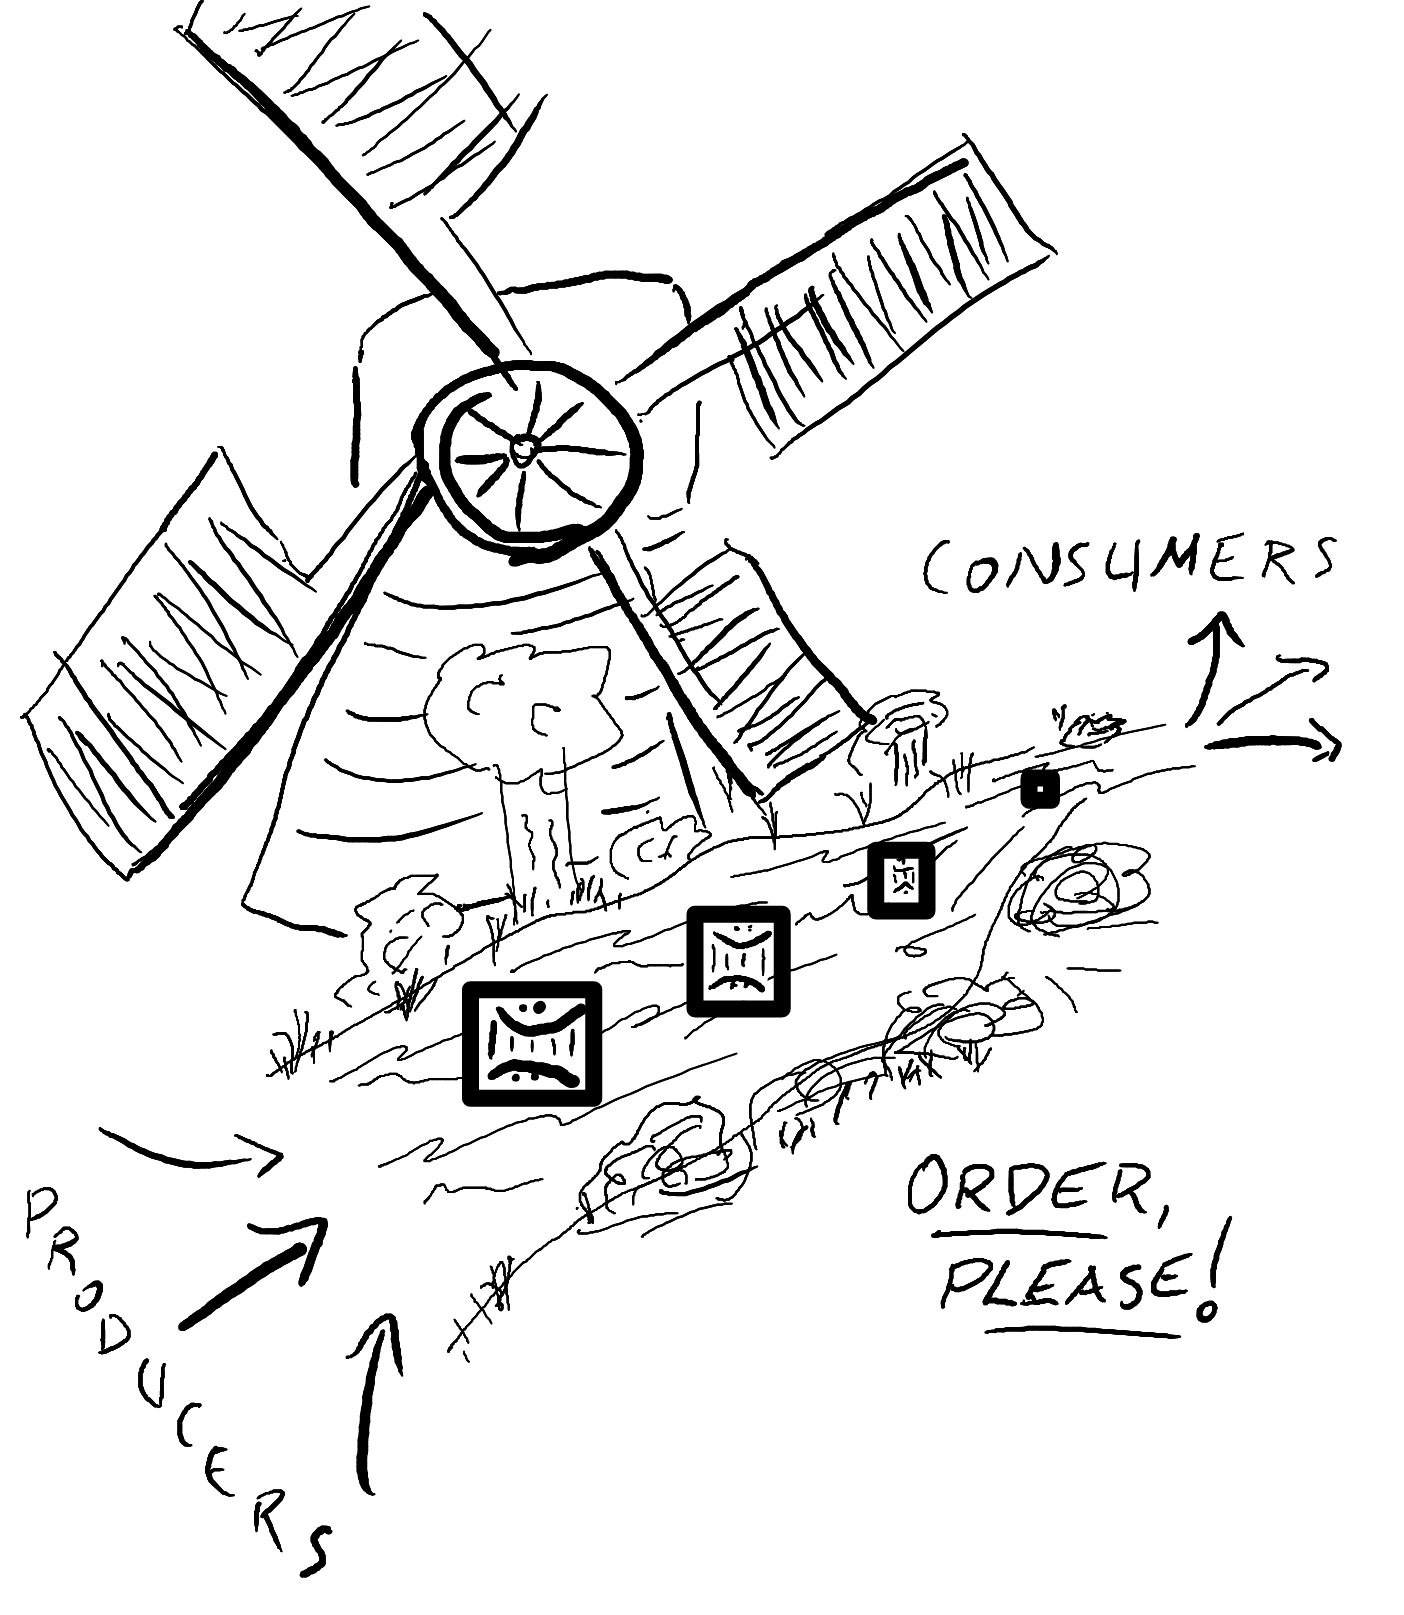
\includegraphics[width=6cm]{images/threads_windmill.png}}
\caption{Ye olde age of Newtonian power.}
\label{fig:windmill}
\end{figure}

to the atomic age!

\begin{figure}[h]
\centerline{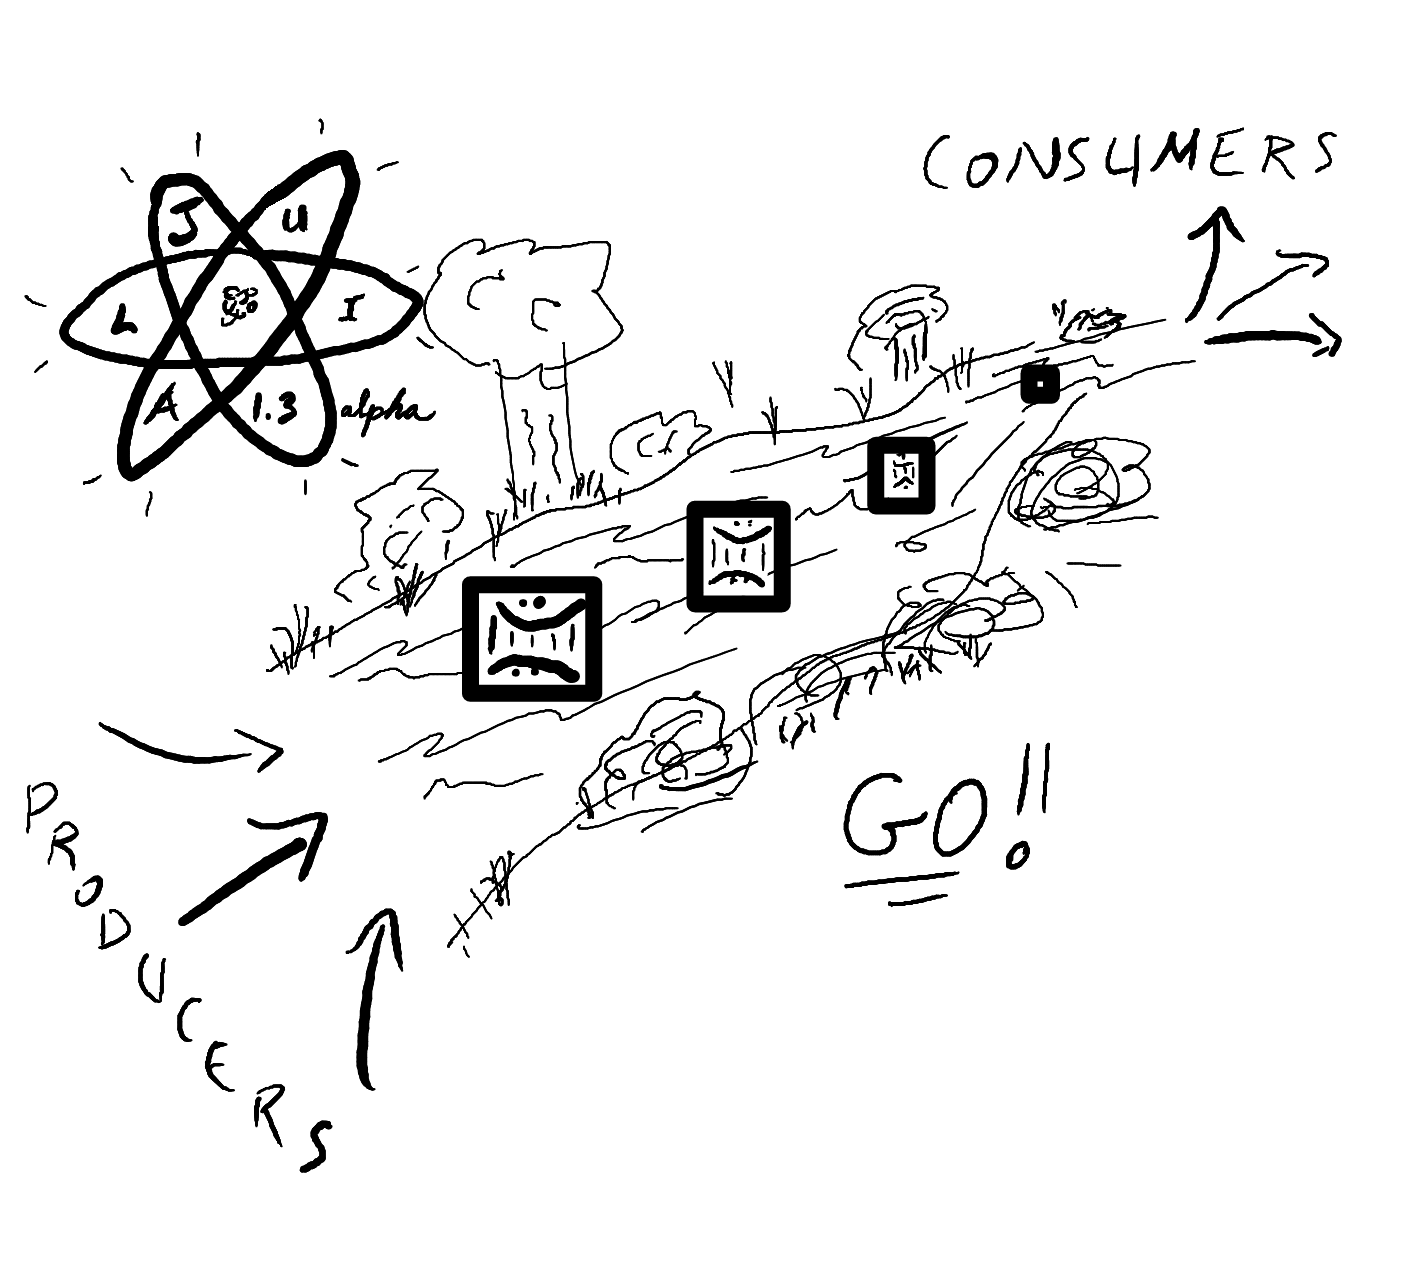
\includegraphics[width=6cm]{images/threads_atomic.png}}
\caption{The atomic age.}
\label{fig:atomic}
\end{figure}


The figure \ref{fig:windmill} is a windmill.
The figure \ref{fig:atomic} is a atom.

% **************GENERATED FILE, DO NOT EDIT**************

\bibliographystyle{juliacon}
\bibliography{ref.bib}


\end{document}
